\section{La guilde des Voleurs}

La guilde des voleurs consiste en réalité en une alliance de divers groupes 
clandestins opérant dans et autour de la ville de Sichua. La guilde est 
localisée dans des sous terrains se trouvant sous la colline des nobles
avec des accès à la fois vers la cote, les quartiers suds et les quartiers 
plus riches directement au dessus du complexe (voir carte). La guilde est
dirigée par huit maîtres: le maître assassin, le maître comptable, le maître 
esclavagiste, le maître escroc, le maître racketteur, le maître pirate, le 
maître voleur et la grande maîtresse (sous-entendu des prostituées). Ces huits 
dirigeants sont en charge des huits activités criminelles de la guilde et
s'occupent de la coordination entre les différentes branches. Le leader
de la guilde est généralement le maître assassin, un personnage 
particulièrement mystèrieux connu seulements des autres maîtres à la
tête d'un groupe de meurtrier aussi efficaces que discrets.


\begin{figure*}[p]
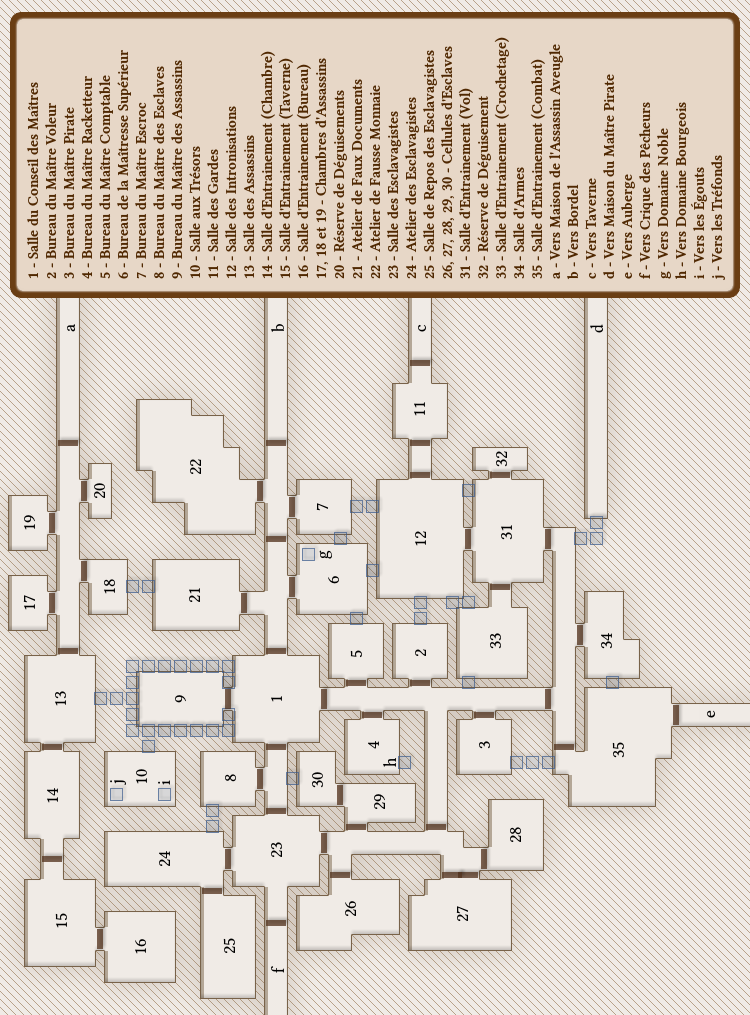
\includegraphics[width=16cm]{Maps/GuildeVoleurs.png}
\end{figure*}

\subsection{Les Différentes Branches}

\subsubsection{Les Groupes Locaux}

La ville de Sichua est en fait occupée en grande partie par des groupes
semi-indépendants ayant prété allégence à la guilde. Ceux-ci font appels 
à la guilde pour recevoir des renforts en cas de besoins ou de préparation 
d'un gros coup, mais doivent aussi s'aquitter d'une taxe auprès de celle-ci. Ils dépendent
d'un maître différent en fonction de leur localisation géographique:
l'ile de la source au maître assassin, le quartier des marchés au maître
comptable, le quartier du port sud au maître esclavagiste, le quartier 
bourgeois au maître escroc, le quartier pauvre du sud au maître racketteur,
le quartier du port nord au maître pirate, les quartiers nords au maître 
voleur et le quartier noble à la grande maîtresse. Cette dépendence hiérarchique 
n'empèche bien sur pas chaque groupe local de pratiquer n'importe lesquelles des huits
activités. Néanmoins, il est clair que ces groupes de petites frappes ne sont
jamais vraiment très puissant. 

Les groupes locaux ne couvrent néanmoins pas tout le territoire de la ville
et un certain nombre d'agents de la guilde dépendent directement d'un maître.
Ceux-ci sont en général les meilleurs agents des groupes locaux et sont recrutés
par la guilde pour s'occuper des affaires les plus lucratives directement. 
Les plus expérimentés obtenant finalement la direction d'un groupe local
si ils survivent suffisamment longtemps dans le milieu. Les chefs de groupe
locaux ont aussi un pouvoir important pour nominer un nouveau maître
lorsque l'ancien disparait. Ils décident alors de la promotion de l'un d'entre 
eux au rang de maître. Il est a noté qu'aucun groupe de malfrats n'est connu 
sur l'île de la source, le système de promotion du maître assassin échappe donc
à cette règle, mais reste un mystère pour le reste de la guilde.

%Liens vers groupe évoqué dans la quête ?


\subsubsection{Les Faussaires}

Dans le complexe de la guilde se trouvent deux ateliers important, l'un
accueillant de véritables artistes experts en conception de faux documents
et en imitations de signatures et l'autre est dédié à la fabrication de fausses 
monnaies. Le maître comptable est en charge de l'exploitation des ces deux
ateliers et de la diffusion de leurs produits. La fabrication de faux en
particulier est généralement utilisé pour des escroqueries de haut niveau
permettant souvent de voler de véritables fortunes.

Le maître comptable est un riche marchand qui tient un rôle clef pour
le blanchiment des entrées d'argent de la guilde dans son ensemble.
...

\subsubsection{Les Esclavagistes}

L'esclavagisme est interdit à Sichua, néanmoins il est possible d'y transferer
et d'y vendre vos esclaves si vous avez de bons contacts. Les esclavagistes 
utilisent une petite crique discrète dans le sud de Sichua pour transférer
les esclaves qui sont gardés directement dans les sous terrains de la guilde.
Ceux-ci seront exportés ensuite vers des îles loin au sud de Sichua, où la
pratique est légale. 

Le maître esclavagiste est un riche ...

\subsubsection{Les Escrocs}

Les escrocs de la guilde ont des activités multiples dans les jeux d'argents
généralement truqués. Ce groupe a aussi un rôle majeur dans le recel des 
marchandises volées par les autres branches de la guilde.

Le maître escroc est Meribald Dalloris (page \pageref{MeribaldDalloris}).

\subsubsection{Les Racketteurs}

Le principal rôle de ce groupe est de lever des "taxes" sur les marchands 
des quartiers les plus pauvres. Ils servent aussi de force de maintien de 
l'ordre à l'interieur de la guilde et peuvent être solicités pour remettre 
un groupe local sur la bonne voie. Enfin cette armée interne est parfois 
utilisée contre des concurents tentant de s'introduire dans la ville. 

\subsubsection{Les Pirates}

La piraterie dans les environs de Sichua a été éradiquée depuis longtemps,
néanmoins les navires marchands traversant l'océan des confins du nord au sud
crée une attraction irrésistible pour les loups de mer de tous horizons qui
guèttent leur proies potentiel au large du désert des ombres. Le grand dragon 
rouge Tarkin règne sur la région gardant les puissantes frégates de Sichua a
distance. Les pirates quand à eux prennent le risque... à moins qu'ils aient 
un accord avec le dragon et lui paye un droit de passage? 

Quoiqu'il en soit Sichua est le plus grand marché de la région et donc un lieu 
tout naturel pour écouler les marchandises accumulées. Le maître pirate est ainsi
plus un passeur qu'un véritable pirate et il sert de principalement de lien entre 
les pirates et le réseau de recelleurs de la guilde. La guilde de Sichua est aussi
le lieu où il peut vendre ses prisonniers comme esclave, optimisant ainsi ses 
voyages. 

Officiellement le maître pirate et ses hommes son équipage tout ce qu'il y a de 
plus respectable. Le maître pirate étant même un armateur important de la ville
avec de nombreuses connexions à la prévoté des marchands.


\subsubsection{Les Voleurs}

Les voleurs forment le c\oe{}ur de métier de la guilde et lui ont donné leur 
nom, mais cela fait bien longtemps qu'ils ont compris que parmis les diverses 
activitées clandestines pratiquée en ville se n'ést pas la plus rentable. Ils
ont reussit à tirer leur épingle du jeu en investissant les sous-terrains du
quartier noble et en dérobant il y a de nombreuses année le puissant artefact 
nain nommé "Keram Dek" ou "Pierre de Tranquilité". Celle-ci fut construite en 
des temps immémoriaux par les nains de la région pour empêcher les incursions
des races étrangères, en particulier en provenance des tréfonds.

Les voleurs de la guilde gardent un rôle important pour le recrutement au sein
de la guilde. Les plus doué des assassins et des faussaires de la guilde furent
ainsi tous recrutés enfant alors qu'ils pratiquaient de menus larçins sur un marché 
ou dans une taverne malfamée. Beaucoup de voleur se reconvertissent ainsi en
vieillissant pour mettre leur dextérité au services de travaux plus rentables...

Une petite partie des voleurs expérimentés rèstent néanmoins dans le groupe,
ils se chargent des cambriolages les plus complexes. C'est généralement le maître
voleur qui agit comme leader de cette équipe qui garde encore une grande fierté
d'être les descendants spirituels de ceux qui dérobèrent autrefois le Keram Dek. 

\subsubsection{Les Prostituées}

Alors que les prostituées furent longtemps exploitées par les racketteurs, elles 
ont finallement su trouver une place au sein de la guilde grâce à certaines d'entres
elles qui surent trouver des alliés au seins des autres factions de la guilde.
Celle-ci apprirent pour ce faire à exploiter les precieuses informations qui leur 
sont confiées par leur clients. A présent le rôle principal des prostituées dans la
guilde est de fournir les noms de riches personnages ayant des meurs particulièrement
aux racketteurs et escrocs, qui se chargent ensuite de faire fructifier ses 
informations. Les prostituées servent aussi souvent à isoler une proie pour un vol, 
voir même un assassinat. La rumeur dit même que certains assassins serait infiltré
parmis les prostitués. Point difficile à verifier tant le groupe des assassins de
la guilde est secret.

\subsubsection{Les Assassins}

Les assassins recrutent leurs hommes au sein de la guilde dans son ensemble,
recherchant les plus doués, mais aussi les plus taiseux et les moins alcoolisés.
Les rares sélectionnés restent généralement membre de leur anciens groupes mais
réduisent progressivement leurs activités alors qu'ils sont entrainés à l'art 
de tuer sans être vu... Il y a peut à dire à propos de ce groupe tant il est 
secret, à part qu'ils sont pret à prendre n'importe quel nom! Y compris celui
du duc lui même pourvu qu'on y mette le prix. 

\subsection{Rapports à l'Exterieurs}

Un accord secret avec les Alchimistes

Sert de source d'information à certains dirigeants

Siège au conseil des cinq

\subsection{Géographie de la Guilde}

\paragraph{1. Salle du Conseil} Relativement grande salle voutée, elle comporte une
lourde table en bois entourée de chaises. Avec de lordes portes dans chaque mur.
Sous la table de la salle du conseil de la guilde des voleurs se trouve une stèle
de pierre gravée de runes naines émanant un pouvoir magique puissant. C'est un 
puissant artefact de dissimulation et de répulsion qui empêche tout ennemis de 
trouver le chemin menant au lieu qu'il protège. L'objet pèse une centaine de kilo,
mais si les aventuriers s'en emparent, ils permettent aux créatures des tréfonds
de remonter vers le complexe et déclenche une quête annexe pour sceller le túnel
après quelques semaines. Ils doivent ainsi descendre avec un nain expert mineurs 
qui indique ou ebouler le passage pour le bloquer définitivement. 

\paragraph{2. Bureau du Maître Voleur} Petite pièce avec un bureau en son centre.
La salle semble très banale mais comporte plusieurs compartiments secrets, à la 
fois dans le bureau et et dans certains murs. Le plus important d'entre eux étant
un passage vers un des balcons de la salle des intronisations. Les compartiments
secrets nécessite un jet d'investigation DC 20 pour être trouvé (faire 3 jets, 
bureau, coffres, passage), un jet DC 15 d'outils de voleurs pour être dévérouillé.
Si le joueur cherche, il découvre néanmoins que les passages sont piégés avec un 
jet de investigation DC 10, il peut aussi s'en appercevoir avec une perception 
passive de 15 ou plus. Dans le coffre se trouvent une amulette d'anti-détection,
des chaussons d'araignée et 3000 PO. Dans le bureau se trouve un anneau de saut et
un anneau d'action libre.

\paragraph{3. Bureau du Maître Pirate}
Cape de Raie Manta, yeux de lynx, 1500 PO

\paragraph{4. Bureau du Maître Racketteur}
Flute de hantise, gantelet de puissance d'ogre, 800 PO

\paragraph{5. Bureau du Maître Comptable}
Lanterne révélarice, yeux grossissants, 2000 PO

\paragraph{6. Bureau de la Maîtresse Supérieur}
Éventail enchanté, philtre d'amour x 3, potion de longévité, 500 PO

\paragraph{7. Bureau du Maître Éscroc}
Casque de Télépathie, poussière de disparition, 1200 PO

\paragraph{8. Bureau du Maître des Esclaves}
Chaines dimensionnelles x 2, sceptre tentacule, 250 PO

\paragraph{9. Bureau du Maître Assassin}
Tentures tout autour de la pièce derrière lesquelles on peut se dissimuler. 
Le maître assassin l'utilise et tente même de s'enfuir si les choses tournent 
mal.
Dague vicieuse, Cape de l'araignée, Cimeterre de rapidité, 2000 PO

\paragraph{10. Salle aux Trésors}
Gants de Combat (+1 et permet de ne faire aucun bruit lors des impacts pour
un combat a main nue, ajouter des propriété à débloquer), flêche mortelle 
pour humain, Manuel de coordination physique (pas encore utilisable à chaque 
séance un dé 20, sur un 20 le manuel est de nouveau utilisable!)
12500 PO (+ 7500 PO fausse perception passive DC 13)

\paragraph{11. }
\paragraph{12. }
\paragraph{13. }
\paragraph{14. }
\paragraph{15. }
\paragraph{16. }
\paragraph{17. }
Chambre d'Anderil, assassin d'hérinard. Une fiole de poison des enfers 
à demi vide sur le 
bureau posé sur un plan du temple de la justice permet de le déduire.
Possède une épée sanglante qui explique la marre de sang dans laquelle 
herinard fut retrouvé. Il discute avec un autre assassin du meurtre quand 
les joueurs arrivent. Ils peuvent entendre la conversation à travers la porte.


\paragraph{18. }
\paragraph{19. }
\paragraph{20. }
\paragraph{21. }


\paragraph{22. }
2500 PO de fausse monnaie.

\paragraph{23. }
\paragraph{24. }
Salle de travail, il y a un braséro et un fer de marquage. 

\paragraph{25. }
\paragraph{26. }
Divers esclaves Nain des Montagnes du sud.

\paragraph{27. }
Divers gnomes des roches du désert très au nord.

\paragraph{28. }
Un diable.

\paragraph{29. }
\paragraph{30. }
Le maître des esclaves original. Il est furieux car le maître assassin utilise 
sa marchandise pour invoquer des démons.

\paragraph{31. }
\paragraph{32. }
\paragraph{33. }
\paragraph{34. }
\paragraph{35. }

\paragraph{a. }
\paragraph{b. }
\paragraph{c. }
\paragraph{d. }
\paragraph{e. }
\paragraph{f. }
\paragraph{g. }
\paragraph{h. }
\paragraph{i. }
\paragraph{j. }



